\tableofcontents
\newpage

\section{Введение}
Современная индустрия разработки программного обеспечения развивается очень высокими темпами. Это выражается как в сокращении временного интервала между выпусками новых версий программных продуктов, так и в значительном увеличении числа целевых программных и аппаратных платформ. В качестве основных факторов, повлиявших на темпы развития отрасли, можно назвать следующие:

активное расширение рынка мобильных устройств, открывающее перед разработчиками возможность значительно расширить аудиторию пользователей собственных продуктов;
конкуренция на рынке настольных операционных систем, вследствие которой все большее количество пользователей устанавливает на свои компьютеры не Microsoft Windows, а альтернативные ОС, например на основе ядра Linux;
повышение доступности сети Интернет, позволяющее разработчикам в короткие сроки распространять обновления своих программных продуктов.

Исходя из этих факторов, можно сделать вывод, что наибольшего успеха могут добиваться разработчики, предлагающие свои программные продукты для нескольких программных и аппаратных платформ, и способные в короткие сроки выпускать новые версии своих продуктов. В связи с этим возникает проблема обеспечения поддержки продуктом сразу нескольких платформ.
Проблема поддержки нескольких программных и аппаратных платформ может быть решена следующими способами:
созданием платформо-независимого программного слоя и использованием систем конфигурационного управления или систем сборки ПО, способных обеспечить сборку программы для различных платформ из единой кодовой базы;
использованием платформо-независимых языков программирования и сред исполнения, например Java;
осуществлением портирования продукта на новую платформу.

Первый подход достаточно трудоемок и требует от разработчиков предварительного исследования особенностей возможных целевых платформ. Разработка и поддержка платформо-независимого программного слоя требуют дополнительных трудозатрат и могут увеличить сроки и бюджет разработки. Этот подход может успешно применяться в крупных компаниях, имеющих отдел исследований и несколько отделов разработки, которые позволяют им сократить время разработки программного слоя и окупить разработку слоя за счет его использования в линейке собственных программных продуктов.
Второй подход наиболее прост для разработчиков, но имеет недостатки. Для языка Java основными недостатками являются недоступность среды исполнения Java для всех платформ и различия в программных интерфейсах платформо-зависимых библиотек. Определенных успехов достигло использование интерпретируемых языков программирования, интерпретаторы которых доступны практически на всех платформах. К сожалению, чаще всего интерпретатор предоставляет доступ только к стандартной библиотеке языка, а эффективность исполнения интерпретируемого кода достаточно низка. Это не позволяет использовать такие языки для работы со сложными и нестандартными форматами данных и значительно ограничивает функциональность программ. Исходя из этого можно сказать, что в чистом виде данный подход может быть применен только для использования на различных платформах платформо-независимой бизнеслогики приложения.
Третий подход предполагает адаптацию программы или её компонента, с целью обеспечения их работы в среде, отличающейся от среды, для которой изначально создавалась программа, при этом сохранения функциональность и пользовательские качества оригинальной программы. Портирование позволяет расширять список целевых платформ по мере необходимости и позволяет на ранних этапах разработки не задумываться о поддержке всего многообразия платформ. Процесс портирования требует от программиста высокой квалификации и понимания принципов работы оригинальной программы, а также дополнительных временных затрат на проверку качества полученной программы.
При обновлении версий используемых программой библиотек, изза потери обратной совместимости, могут возникать задачи сходные с задачей портирования и они также могут быть решены с помощью технологий, применяемых при портировании.

Целью данной работы является разработка технологии автоматизации портирования программ при миграции в новое библиотечное окружение. Подобная технология позволит упростить процесс портирования и сократить затраты на его проведение.
Работа организована следующим образом: в первом разделе рассматриваются существующие подходы к автоматизации реинжиниринга программного обеспечения. Во втором разделе выполняется постановка задачи на разработку технологии портирования, определяются ограничения, и делается выбор способа решения. В третьем разделе описывается предлагаемый подход к портированию программ на основе частичных поведенческих спецификаций. В четвертом разделе описывается практическая реализация разработанной технологии портирования. В пятом разделе описываются этапы и результаты тестирования прототипа и его компонентов, и производится анализ полученных результатов.

\section{Обзор методов миграции программ}
Существующие подходы к проблеме миграции программ можно разделить на следующие группы:
\begin{itemize}
	\item Эмуляторы
	\item Трансляторы вызовов
	\item Обёртки (wrappers)
	\item Синтаксические подходы
	\item Семантические подходы
\end{itemize}

Первые три группы можно отнести к динамическим подходам, а оставшиеся две группы - к статическим.

\subsection{Эмуляция}
Эмуля́ция (англ. emulation) в вычислительной технике — комплекс программных, аппаратных средств или их сочетание, предназначенное для копирования (или эмулирования) функций одной вычислительной системы (гостя) на другой, отличной от первой, вычислительной системе (хосте) таким образом, чтобы эмулированное поведение как можно ближе соответствовало поведению оригинальной системы (гостя).

\subsection{Трансляция вызовов}
Благодаря распространённости ОС Windows на сегодняшнем рынке очень многочисленны приложения, разработанные для этой платформы1. Однако зависимость коммерческого приложения от определённой платформы (ОС) может быть не всегда удобной или выгодной. На этот случай существуют средства, позволяющие программам, разработанным для ОС Windows, работать в другой операционной системе. Одним из наиболее развитых среди подобных средств является WINE.

WINE (Wine Is Not Emulator) не является эмулятором операционной системы: то есть он не создаёт изолированной среды для выполнения и не обеспечивает доступ к низкоуровневым системным ресурсам, таким как непосредственный доступ к оборудованию. Функция WINE состоит в том, чтобы, с одной стороны, предоставить win-приложению Win API — стандартный системный интерфейс операционных систем Windows, а с другой стороны, транслировать запросы win-приложения в соответствующие системные вызовы (Unix API). WINE работает на различных Unix-системах, в том числе на Linux. Таким образом, WINE — это своеобразная «прослойка» совместимости между win-приложениями и host-системой2.

Хотелось бы отметить, что процесс WINE всегда выполняется в непривилегированном режиме и не требует никакой модификации ядра операционной системы (в том числе динамически загружаемых модулей). Отсюда следует простой вывод относительно безопасности: любые проблемы, которые могут быть вызваны запуском win-приложений, будут ограничены правами доступа того пользователя, который запустил WINE. В результате win-приложения будут подчиняться политике доступа UNIX-системы и не смогут её нарушать.

У данного ограничения есть и другая практическая сторона: в WINE нет поддержки низкоуровневого обращения к оборудованию (драйверов оборудования, прямой работы с USB-устройствами). Всё периферийное оборудование следует подключать и настраивать в host-системе: для win-приложений эти устройства могут быть доступны стандартным способом через файловую систему или другие стандартные интерфейсы (например, TWAIN для сканеров, который реализован в WINE как обёртка над библиотекой SANE).

Наиболее распространённый способ применения WINE — запуск двоичных win-приложений в Unix-среде. Удобство заключается в том, что при этом не требуется никак изменять приложение — один и тот же вариант годится и для Windows, и для WINE.

Другое, на сегодняшний день пользующееся незаслуженно меньшей популярностью применение — с помощью WINE разработчики ПО могут компилировать свои win-приложения из исходных текстов непосредственно в двоичные исполняемые файлы для Unix. Опять-таки, это те же самые исходные тексты, из которых компилируются двоичные файлы для Windows.

Третий способ использования — WINE позволяет скомпилировать win-приложение из исходных текстов в исполняемый exe-файл, который будет работать на любой Windows-системе.

WINE состоит из нескольких компонент, которые условно можно поделить на три части:

libwine
Библиотека, предоставляющая Win API для win-приложений. По количеству предоставляемых функций её можно сравнить с Qt — столь широк спектр предлагаемых вызовов: от операций с файлами до построения графического интерфейса и обращения к базам данных.
wine
Среда для исполнения двоичных win-приложений, предоставляет программам окружение, неотличимое от Windows. Это окружение помимо Win API включает реестр, стандартные каталоги и файлы. Реестр является единственной изменяемой информацией, необходимой для работы WINE и win-приложений в нём.
утилиты
Утилиты, имитирующие некоторые стандартные win-приложения: текстовый редактор (блокнот), файловый браузер и т. п. Средства компиляции и отладки: имеются заголовочные файлы, которые описывают доступное API, компилятор winegcc, представляющий собой обёртку над gcc, отладчик winedbg и прочие вспомогательные утилиты.

WINE — это свободный проект, который был начат в 1993 году. На тот момент распространённой платформой была Win16 (Windows 3.1), на неё и был ориентирован WINE, на сегодняшний день основным русло разработки — Win32. Исходные тексты WINE выпускаются под лицензией LGPL (Lesser GPL), никаких ограничений по доступу к исходным текстам и их модификации не имеется. WINE снабжён достаточно вразумительной документацией, имеется ряд списков рассылки (англоязычных), как для пользователей, так и для разработчиков, где оперативно решаются любые вопросы.

\subsection{Обертки}

Cygwin

\subsection{Синтаксический подход}
Синтаксические подходы в процессе трансформации используют синтаксические свойства программ. С использованием таких подходов связаны основные достижения в области трансформации программ. К этой группе относятся подходы на основе шаблонных преобразований и перезаписи термов.
В подходах, основанных на шаблонных преобразованиях, по исходному коду строится модель, и определяются шаблоны заменяемого кода. В процессе трансформации осуществляется поиск кода по шаблону и применение к нему трансформаций. Основными различиями в таких подходах являются используемые модели кода, языки описания шаблонов и способы задания трансформаций. Примерами средств на основе шаблонных преобразований могут служить системы ReSharper и Inject/J.

В интегрированной среде разработки IntelliJ IDEA имеется встроенный статический анализатор\cite{ideaStatic}, который непрерывно анализирует код и при наличии предупреждений сообщает об этом пользователю (подсвечивая соответствующий участок кода жёлтым цветом). При этом пользователь может вызвать меню <<Quick Fix>>, которое содержит список предлагаемых исправлений. На рисунке \ref{fig:idea} изображён пример использования этих возможностей IDEA.

Таким образом, эту систему можно охарактеризовать как автоматизированную, а не автоматическую, что сразу меняет сферу применения. Ещё одна важная особенности рассматриваемого инструмента - тот факт, что статический анализатор глубоко интегрирован в систему модификации кода, благодаря чему с высокой точностью определяется место, где необходимо применить исправление.

\begin{figure}[htbp]
	\centering
	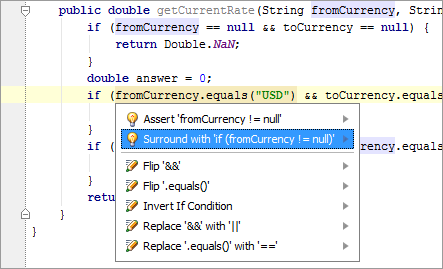
\includegraphics[width=0.8\textwidth]{code_analysis_bugs.png}
	\caption{Предупреждение от статического анализатора в IntelliJ IDEA и всплывающее меню Quick Fix}%
	\label{fig:idea}
\end{figure}

Довольно большое количество исправлений изначально содержится в IDEA, однако имеется возможность добавить свои шаблоны с помощью функции Structural Search and Replace\cite{ideaSSR}. Данная функция во многом похожа на обычный диалог замены текста (Search and Replace), однако учитывает синтаксис и семантику кода. Например, при поиске вхождения не учитывается разница в форматировании между шаблоном поиска и исходным кодом, а также не учитывается порядок объявления членов при поиске класса.

Если нет необходимости искать точное совпадение, в шаблоне можно использовать переменные, в таком случае в указанном месте может быть произвольный текст. Переменные обозначаются с помощью двух знаков \$, как на рисунке \ref{fig:ssr}.

\begin{figure}[H]
	\centering
	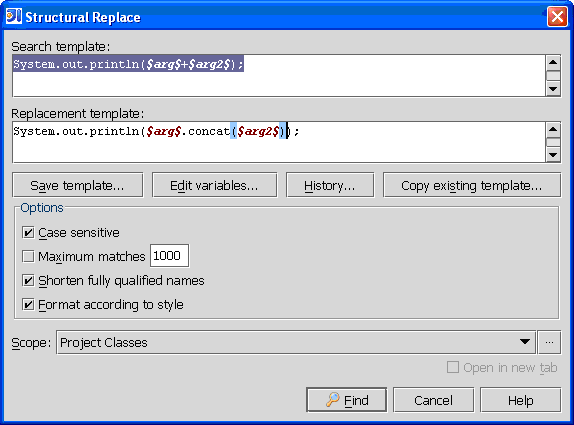
\includegraphics[width=0.8\textwidth]{ssr.png}
	\caption{Пример использования переменных в шаблонах поиска}%
	\label{fig:ssr}
\end{figure}

При этом есть возможность указывать ограничения для каждой переменной: регулярное выражение, которому она должна соответствовать, минимальное и максимальное число элементов программы, которые могут входить в переменную, и так далее.

Большинство синтаксических методов основывается на использовании правил перезаписи. Абстрактная система перезаписи включает множество объектов, над которыми выполняется перезапись, и множество отношений, которые задают возможные преобразования элементов множества объектов друг в друга. Одним из представителей этой группы является язык TXL [3]. В его основе лежит система перезаписи термов, взаимодействие с которой осуществляется с помощью специального функционального языка программирования. Для задания отношений и правила перезаписи задаются на этом языке, а для задания множества объектов в TXL используется расширенная форма Бэкуса — Наура.

Развитием подхода правил перезаписи является концепция стратегий перезаписи. Данная концепция легла в основу языка трансформации Stratego, реализованного в рамках системы Stratego/XT [4]. В данной системе в качестве модели программы, над которой выполняется трансформации, используются аннотированные термы. Таким образом, при построении абстрактного синтаксического дерева программы система получает дополнительно информацию о семантике терма, которая затем может быть использована в правилах перезаписи.

\subsection{Семантические подходы}
\begin{figure}[htbp]
	\centering
	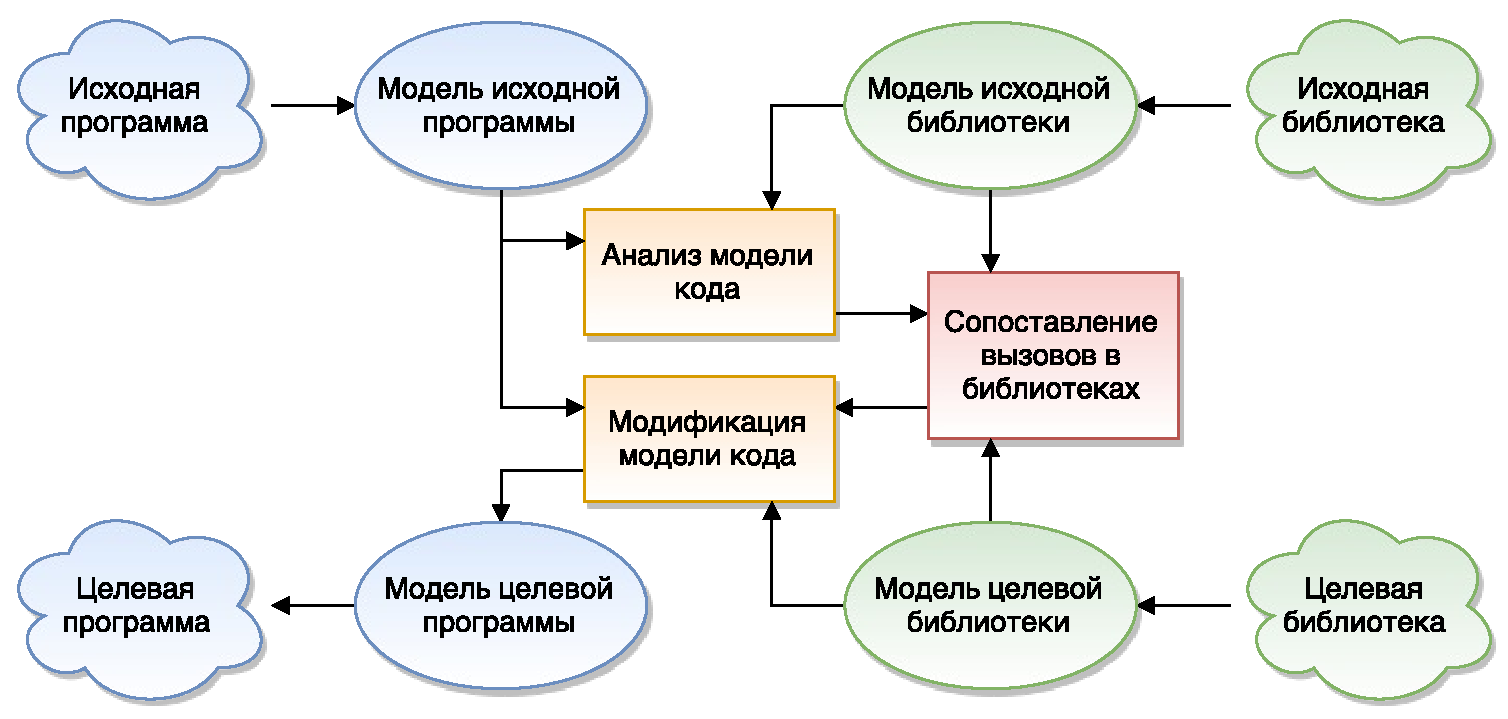
\includegraphics[width=\textwidth]{scheme.pdf}
	\caption{}
\end{figure}

Семантические подходы в основном используются при автоматизации миграции программ с одного языка программирования на другой. Средства данной группы чаще всего применяются при необходимости переноса программ с устаревших языков на более новые. Также эти средства применяются для автоматизации переноса бизнес-логики больших систем на альтернативную программную платформу.
При анализе кода программы средства данной группы могут извлекать информацию о семантике библиотечных вызовов либо из исходного кода библиотек, что не всегда возможно обеспечить, либо из объектных файлов библиотеки. Зачастую полученная в результате семантика вызова подпрограмм библиотеки содержит множество информации связанной с реализацией конкретной библиотеки, а не с тем, что она на самом деле делает. Из-за этого такие средства ограничиваются анализом кода, не использующего или использующего ограниченный набор внешних библиотек с хорошо известной семантикой. Примером такого средства может служить J2ObjC [5]. Это сред ство предназначено для трансляции кода на языке Java в код на языке Objective-C для платформы iOS. Основным применением средства является совместное использование бизнес-логики и логики доступа к данным, описанной на языке Java, на различных платформах, таких как Android и iOS. Средство позволяет использовать в коде многие возможности Java, такие как потоки, исключения, анонимные классы и рефлексию. Также оно позволяет транслировать использующие библиотеку JUnit модульные тесты. На текущий момент проект находится на ранней стадии развития и поддержка других внешних библиотек
не реализована.

Еще одним примером может служить средство Emscripten [6]. Оно позволяет транслировать байткод LLVM в код на языке JavaScript. С помощью данного средства было портированно много крупных проектов с открытым исходным кодом. Байткод LLVM может быть получен из языков C, C++, Objective-C и др. с помощью компиляторов GCC и Clang. Байткод может быть получен из скомпилированной версии библиотеки, но при этом в нем нет информации о том, из чего байткод был получен, что позволяет средству генерировать только однофайловые программы.

\section{Обзор инструментов миграции программ}
Инструмент миграции программ является частным случаем транспайлера (transpiler, transcompiler, source-to-source compiler) - компилятора, результатом работы которого является код на высокоуровневом языке (в отличие от обычных компиляторов, которые на выходе дают программу в машинных кодах или на языке ассемблера). Помимо миграции, транспайлеры используются для решения следующих задач:

\begin{itemize}
\item Трансляция программ на другой язык программирования. Например, первый компилятор языка C++ (Cfront, 1983 г.) являлся именно транспайлером. Сначала программа на C++ транслировалась в программу на C, после чего собиралась одним из существующих компиляторов языка C.
\item Рефакторинг программ (процесс изменения внутренней структуры программы, не затрагивающий её внешнего поведения). Многие современные среды разработки, такие как IntelliJ IDEA или Eclipse, включают в себя системы автоматического рефакторинга программ.
\item Перенос программ на другую версию языка. Пример инструмента для переноса на более новую версию языка - скрипт 2to3, транслирующий программу на языке Python 2 в программу на языке Python 3. Третья версия языка Python не имеет обратной совместимости со второй версии, и поэтому разработчикам необходимо переписывать старые программы, чтобы иметь возможность запускать их на новых версиях интерпретатор. Скрипт 2to3 позволяет во многом автоматизировать перенос. Пример переноса на более старую версию языка - инструмент Babel, позволяющий писать программы на языке ECMAScript 6 и исполнять их, даже если интерпретатор поддерживает только ECMAScript 5 или 3.
\end{itemize}

\section{Выводы}